\begin{activity}{Density and Porosity}

\section*{Purpose}
To develop intuition for how porosity affects rock density and how compaction during burial modifies density contrasts relevant to gravity interpretation. By examining real porosity--depth data, students will identify simple mathematical descriptions of compaction and explore how changes in porosity influence the bulk density of sedimentary rocks.

\section*{Learning Outcomes}

By the end of this activity, you should be able to:
\begin{itemize}
  \item describe how porosity varies with burial depth and explain the role of compaction,
  \item identify a plausible mathematical model for porosity reduction with depth and interpret its parameters,
  \item derive and apply a bulk-density relationship for porous rocks,
  \item explain how compaction alters density contrasts between sedimentary rocks and crystalline basement,
  \item relate density changes caused by porosity loss to qualitative gravity responses.
\end{itemize}

\section*{Introduction}
In week 2, we calculated several physical properties, though in each case we assumed porosity was negligible. However for many rocks, especially sedimentary rocks near the surface, porosity can be significant.

\paragraph{What is porosity?}
Porosity is void space, but that doesn't mean it is empty.  Other than an unsaturated zone at the surface the voids are generally saturated with fluid (water, brine, steam, oil, gas, \ce{H2}). The fraction in sediments can be 30\% for porous sandstone up to $\sim$70\% at the seafloor.  Though for most sedimentary rocks it is $<$20\% and crystalline---plutonic and metamorphic rocks---porosity is often $\lesssim$2\%.  Porosity comes in a few flavors:
\begin{description}
  \item [intergranular] -- between mineral grains, common in sedimentary and volcanic rocks,
  \item [vesicular] -- pore space created by gas bubbles, common in volcanic rocks, particularly shallow erupted basalts,
  \item [fracture] -- cracks and joints created by tectonic activity, decompression near the surface, cooling, or meteorite impacts (minor),
  \item [weathering related] -- generally dissolution by groundwater.
\end{description}
Most porosity loss occurs within the upper $\sim$10--11 km of the crust, where increasing overburden stress closes fractures and compacts sediments. Small amounts of porosity may persist to greater depths.

Porosity is generally reported as a decimal fraction between 0 and 1, or as a percentage of the total volume of the rock.  Only porosity will be reported, not the solid component (matrix), so what fraction makes up the this portion?---well the rest of it of course!

\subsection*{Tasks}

In the figure below you will see sediment porosity--depth data for a chalk section off the coast of Norway.  Estimate the nature of the compaction.
\begin{figure}[ht]
  \centering
  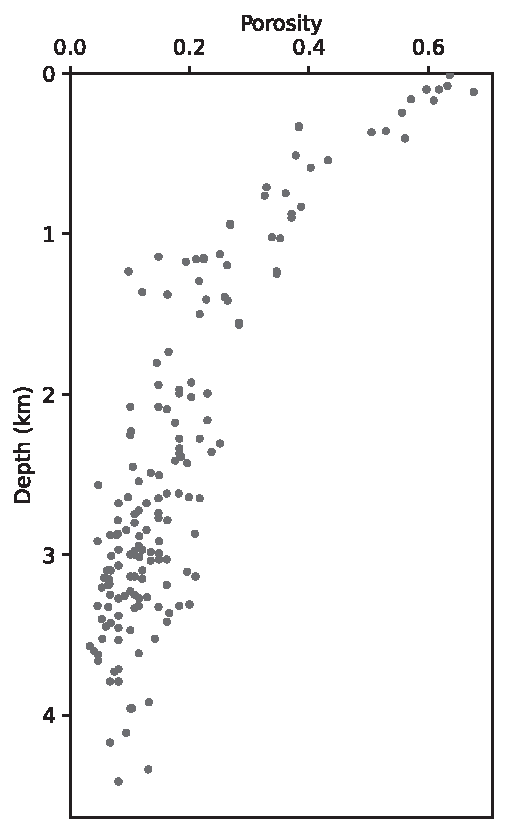
\includegraphics{figures/porosity_depth_data.pdf}
  \caption{Porosity data from Mallon and Swarbrick (2002) on calcareous ooze.}
  \label{fig:sed_porosity}
\end{figure}
\FloatBarrier

\begin{questions}
  \question{Compaction of Sediments}
    To estimate the compaction relatioship with depth, start by drawing an approximate curve for porosity from the surface to 4 km depth.

    Which of the mathematical models appears to fit the data best?  And, why do all of these models include a $z/h$ term?
    \[ 
      \text{a.}\enspace \phi(z) = \phi_0 - z h^{-1} \hspace{3em}
      \text{b.}\enspace \phi(z) = \phi_0 \exp(-z h^{-1}) \hspace{3em}
      \text{c.}\enspace \phi(z) = {\displaystyle\frac{\phi_0}{1 + z h^{-1}}}
    \]
    \answerbox

    \clearpage
    Assuming your preferred model, estimate values for $\phi_0$ and $h$? Also label these on the figure on the appropriate axes.
    \answerbox

    What physical meaning would you assign to: (a) $\phi_0$, (b) $h$?
    \answerbox

  \question{Density of Sediments}
    If the density of the matrix material, $\rho_m$, in the chalk examined above ranges from 2650 to \SI{2720}{kg.m^{-3}}, derive a relationship for the bulk density of the sediment with pores filled with seawater ($\rho_f = \SI{1030}{kg.m^{-3}}$).
    \answerbox

    Which depth interval produces the largest change in density: 0--1 km, 1--2 km, 2--3 km, or 3--4 km?  Why?
    \answerbox[36pt]

    What is the density of the sediments at the surface and $h$?  What is the relative change in density?
    \answerbox

  \question{From Porosity to Gravity}
    As sediments become buried and compacted, do you expect the density contrast between the sediments and crystalline basement to increase or decrease?
    \answerbox[24pt]

    What implications does this have for gravity interpretation?
    \answerbox

\end{questions}

\end{activity}